\section{Contextual constraints}
The grammar of Arc is a \gls{cfg} and only expresses the structure of the language. Further contextual constraints are required to specify if a program is well-formed and meaningfully correct. This section describes Arc's contextual constraints: the scope- and type rules.

\subsection{Scope rules}\label{subsec:scoperules}
The scope rules govern visibility, hiding some parts of a program from others. It also rules where certain things are allowed and others are not.

The Arduino language has static scope, with nested and flat block structures~\cite{cppref}. Blocks are declarable within other blocks (nested), but functions within other functions cannot(flat). Arc will have similar scope rules, making compilation more straightforward as source code and target code resemble each other regarding scope.

Arc statements and blocks, therefore, have nested scoping, while function declarations have a flat scope and are not declarable inside a scope. However, one key feature of Arc is its \textit{task} construct, which is not present in Arduino and requires particular focus.

A task declaration is like a function declaration and cannot be inside another scope. Additionally, declaring local variables inside the scope of a task declaration is not possible. The Protothreads implementation does not preserve local variables when a thread becomes blocked, making it hard to know if using local variables in a thread will work as the programmer intended.

Another solution to this problem could be to hoist local variable declarations within a task declaration into the global scope. However, this could make static scopechecking more difficult. Listing~\ref{lst:hoistclash} shows how the hoisting of a locally declared variable may clash with globally declared variables. While the hoisting issue is not unsolvable, it is clearer to disallow variable declarations within a task declaration. Most importantly, writing an Arc task is entirely declarative - tasks are never called, unlike functions.


\begin{listing}[htb!]
    \begin{minted}[label=Scope clash]{text}
        num a = 1;
        task() {
            num a = 2; // hoist causes a clash here
        }
    \end{minted}
    \caption{Example of hoisting that causes a clash.}
    \label{lst:hoistclash}
\end{listing}


\subsubsection{The environment store model}
To describe the static scope rules of Arc with operational semantics, we use the environment-store model from Figure~\ref{fig:envstomodel}. The environment-store model describes variables as binding to locations, and locations binding to values, while the locations and values are then read with partial functions called \textit{environment} and \textit{store}.

Arc has two environments, the variable environment and the function environment. To define the semantics, some functions and sets must be described first.

\begin{table}[htbp]
    \centering
    \begin{tabular}{l}
        \toprule
        $\textbf{Loc} = \mathbb{N} - $ The set of locations                                   \\
        $x \in \textbf{Var} - $ Variables                                                     \\
        $l \in \textbf{Loc} - $ An arbitrary location in \textbf{Loc}                         \\
        $S \in \textbf{Stm} - $ Statements                                                    \\
        next $- $ A special 'pointer' holding the value of the next element in \textbf{Loc}   \\
        new $: \textbf{Loc} \rightarrow \textbf{Loc} - $ function to return succesor location \\
        \bottomrule
    \end{tabular}
    \caption{Sets and function definitions.}
    \label{tab:setsandfunctions}
\end{table}


\begin{equation}\label{eq:environmentset}
    \textbf{Env}_v = \textbf{Var} \cup \{'text{next}\} \rightharpoonup \textbf{Loc}
\end{equation}

\begin{equation}\label{eq:storeset}
    \textbf{Sto} = \textbf{Loc} \rightharpoonup \textbf{Lit}
\end{equation}



\begin{table}[htbp]
    \centering
    \begin{tabular}{ll}
        \toprule
        $[FUNC_{DECL}] $ & $\dfrac
            {env_v \vdash \langle env_f[f \to (stmt, env_v, env_f)] \rangle \to env_f \prime}
            {env_v \vdash \langle \text{func f is stmt; } env_f \rangle \to env_f \prime}$ \\
        \bottomrule
    \end{tabular}
    \caption{Arc's scope defined with operational semantics.}
    \label{tab:arcscoperules}
\end{table}

The sets of these partial functions are described in Equations~\ref{eq:environmentset} and~\ref{eq:storeset}.


where next is bound to the next location, and calculated with new $l = l + 1$ .




\begin{figure}[htbp]
    \centering
    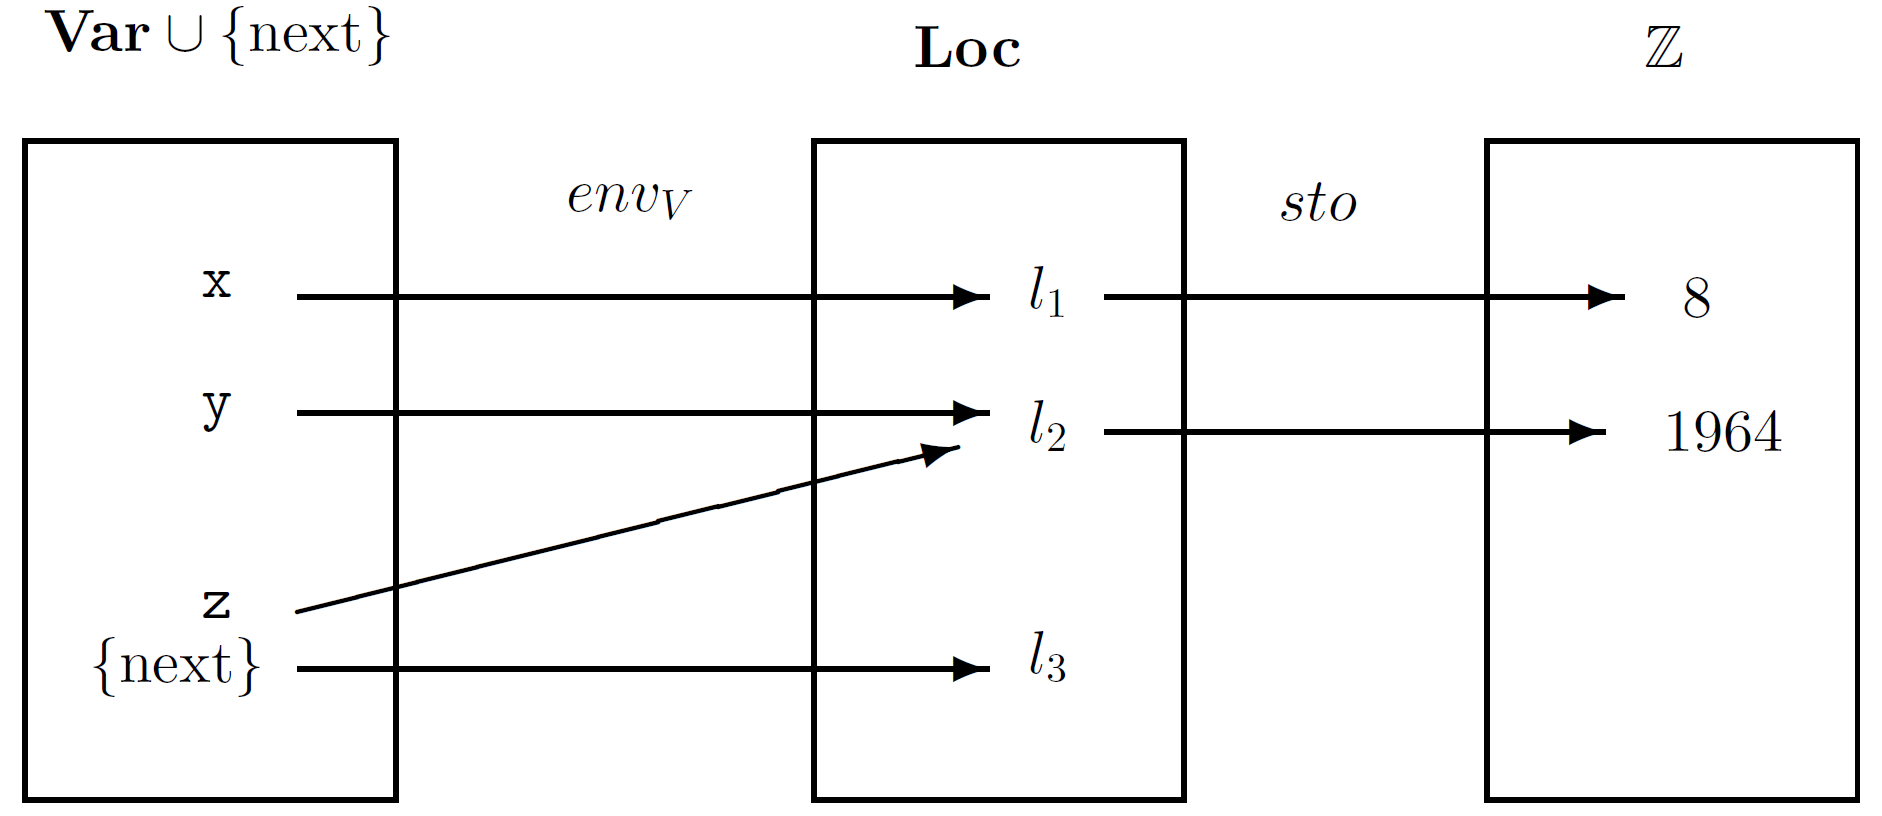
\includegraphics[width=0.8\textwidth]{figures/Environment_Store.png}
    \caption{Example diagram of the environment store model~\cite{Huttel2010}.}
    \label{fig:envstomodel}
\end{figure}


$[if_{true}]
    env_{vf}\langle \text{if expr then stmt}_1 \text{else stmt}_2,sto \rangle \rightarrow env_{vf} \langle stmt_1,sto\rangle$
Where  $env_{vf},sto \vdash expr \to true$



NOTES:

Function call can't use recursion.
Function parameters are call by value.
Task parameters are mutable call by reference, and there can be only one mutable reference at a time.

Can pin declarations and variable declarations be in the same environment?
What environment are tasks stored in, if any? Describe all 3 types.











\begin{figure}[htbp]
    \centering
    \missingfigure{Insert image of scope rules in Arc}
    \caption{Diagram of the scope structure of Arc.}
    \label{fig:arcscoperules}
\end{figure}


@misc{cppref,
    oraganization       = {cppreference},
    url = {https://en.cppreference.com/w/cpp/language/scope},
    title        = {Scope in C++},
    urldate = {2022-02-10}
}